\documentclass{article}
\usepackage{fancyhdr,booktabs}
\usepackage{amsmath}
\usepackage{float}
\usepackage{graphicx}
\usepackage{indentfirst}
\usepackage{geometry}
\usepackage{citesort}

\begin{document}

\section{Introduction}
\section{Numerical Method}
In this section we describes how we generate EMRI waveforms in non-Kerr metric and process EMRI signal. In \ref{p_krz}, a continuously parametrized metric proposed by \cite{KRZ} is introduced, in \ref{p_kludge}, the method to generate EMRI waveforms proposed by \cite{kludge} is described and \ref{p_mf} summarizes the signal processing pipeline.
\subsection{Konoplya-Rezzolla-Zhidenko parametrization}
\label{p_krz}
In order to test Kerr hypothesis or General Relativity, one need an alternative theory or a non-Kerr metric. Here we use the metric parametrization proposed by Konoplya, Rezzolla and Zhidenko (see \cite{KRZ}) and still calculate the gravitational wave within General Relativity. 

The line element around an axisymmetric black hole in KRZ parametrization is \cite{KRZ}:
\begin{equation}
	ds^2=
\end{equation}
Where the functions $Y$ can be expanded by power series of $\cos\theta$. Here we use the same deformation parameter as \cite{cosimoKRZ}, namely $\delta_i, \, i=1,2,3,4,5,6$ related to the metric functions by
\begin{equation}
K=	
\end{equation}

KRZ parametrization preserves stationarity and axisymmetry. When each $\delta_i$ is set to 0, the metric recovers Kerr metric.

\subsection{"Kludge" Waveform}
\label{p_kludge}
We use the method established in \cite{kludge}, i.e. Kludge waveform, to calculate EMRI waveforms. The procedure is: regarding the stellar mass object as a point particle, first calculate the trajectory of the particle in a given metric by integrating geodesic equations; then use quadruple formula to get the gravitational wave from geodesics.

In our instance, to calculate the geodesics, we use:
\begin{equation}
	\dot{u^\mu}=-\Gamma^\mu_{\rho\sigma}u^\rho u^\sigma
\end{equation}
\begin{equation}
	\dot{x^\mu}=u^\mu 
\end{equation}
where $x^\mu$ is the Boyer-Lindquist coordinate of the particle, $u^\mu$ is the 4-velocity and $\Gamma^\mu_{\rho\sigma}$ is Christoffel connection. We didn't use conservation of particle mass, energy and angular momentum to reduce equation but to monitor numerical error. Namely at each step of integration, we check the conservation quantities defined by:
\begin{equation}
	\eta = g_{\mu\nu} u^\mu u^\nu
\end{equation}
\begin{equation}
	E = -u_t = - g_{tt} u^t -g_{t\phi} u^\phi
\end{equation}
\begin{equation}
	Lz = u_\phi = g_{t\phi } u^t + g_{\phi\phi} u^\phi
\end{equation}
 and in Kerr cases, we also check Carter constant
 \begin{equation}
 	Q = (g_{\theta\theta} u^\theta)^2 + \cos ^2 \theta (a^2 (\eta^2-E^2) + (\frac{Lz}{\sin \theta})^2 )
 \end{equation}
During the calculation, we keep the relative drift of conserved quantities less than $10^{-7}$.

Transform $(r,\,\theta,\,\phi)$ into $(x,\,y,\,z)$ with the definition of spherical coordinate (rather than the Boyer-Lindquist coordinate), namely $x=r\sin\theta \cos \phi,\, y=r\sin\theta\sin\phi,\, z=r\cos\theta$. Then use quadruple formula and transform the waveform into transverse-traceless gauge (see formula (17) and (23) in \cite{kludge}). With the resulted "plus" and "cross" components, we define our waveform as $h = h_+ + i h_\times$
\subsection{Matched Filtering}
\label{p_mf}
\section{Confusion Problem}
When we try to identify EMRI signals, the confusion problem, as described in \cite{sameOmg}, could prevent us from discern non-Kerr signal and Kerr signal. An overlap over 0.97 might happen between non-Kerr signals and Kerr ones with proper parameters. In \ref{p_2d} and \ref{p_3d} we show the confusion problem when matching EMRIs from equatorial and inclined orbit 
\subsection{Equatorial orbit}
\label{p_2d}
Given a waveform under spacetime with non-zero deformation parameter, in order to see if there is "confusion problem", we need to decide which waveform under Kerr spacetime is most similar to it and look at their overlap. Here we search for existence confusion problem with similar method as \cite{majorPRD}, i.e. looking at waveforms with same orbital frequency. The orbital frequencies in Kerr spacetime are given in \cite{tauOmg}. In equatorial orbits, there are two frequencies $\omega_\phi$ and $\omega_r$ related to motion of $\phi$ and $r$ coordinates.

\begin{figure}[!htb]
	\centering
	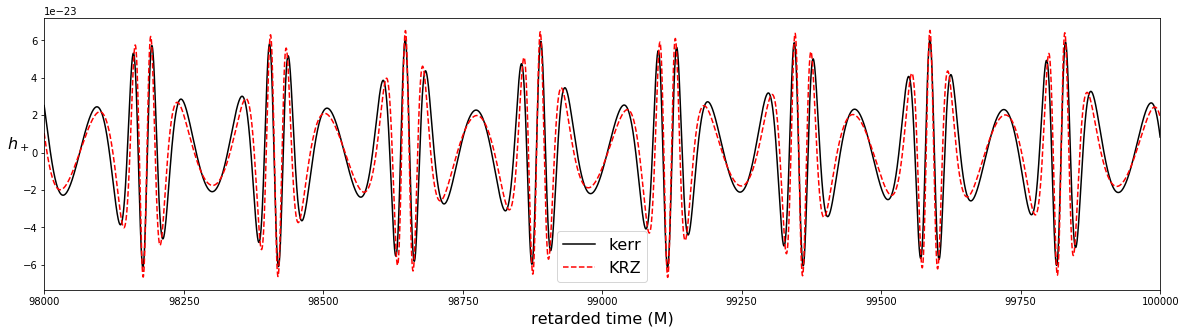
\includegraphics[width=16cm]{krz_kerr_wave.png}
	
	\caption{Comparison between waveforms of $h_+$ with respect to retarded time in units of central black hole mass $M$. The black solid line is the waveform under $\delta_1=0.2$, e=0.5,p=6. The red dashed line is the waveform under $\delta_1=0$ and e, p adapted so that the orbital frequencies with respect to t $\omega^{(t)}_r$ and $\omega^{(t)}_\phi$ are the same as that of the orbit under d1=0.2, e=0.5, p=6. The green dotted line is the waveform under $\delta_1 =0$ and e, p adopted so that $\omega^{(\tau)}$s are the same . The spin of the central black hole is 0.5M.}
	\label{kkwave}
\end{figure}	

If we restrict ourselves to equatorial motion, set the initial $t$ and $\phi$ to 0 in view of stationarity and axisymmetry and set initial $r=r_{max}$, then the orbit is uniquely determined by orbital eccentricity $e$, semilatus rectum $p$, deformation parameters $\delta_i$, BH mass $M$ and BH spin $a$. As described in \cite{majorPRD}, we can achieve same orbital frequency as non-Kerr signal by varying orbital parameters $e, \,p$ or BH parameters $M, \, a$. So we need to consider EMRIs determined by $(\delta,\, a,\, M,\, e,\, p)$, $(0,\, a,\, M,\, e_{Kerr},\, p_{Kerr})$ and $(0,\, a_{Kerr},\, M_{Kerr},\, e,\, p)$. Comparison of waveforms of same orbital frequency is show in Fig. \ref{kkwave}. The overlap between waveforms varying BH mass and spin is over 0.99. In fact, the geodesics that generate the two waves are overlapping.  

\begin{figure}[]
	\centering
	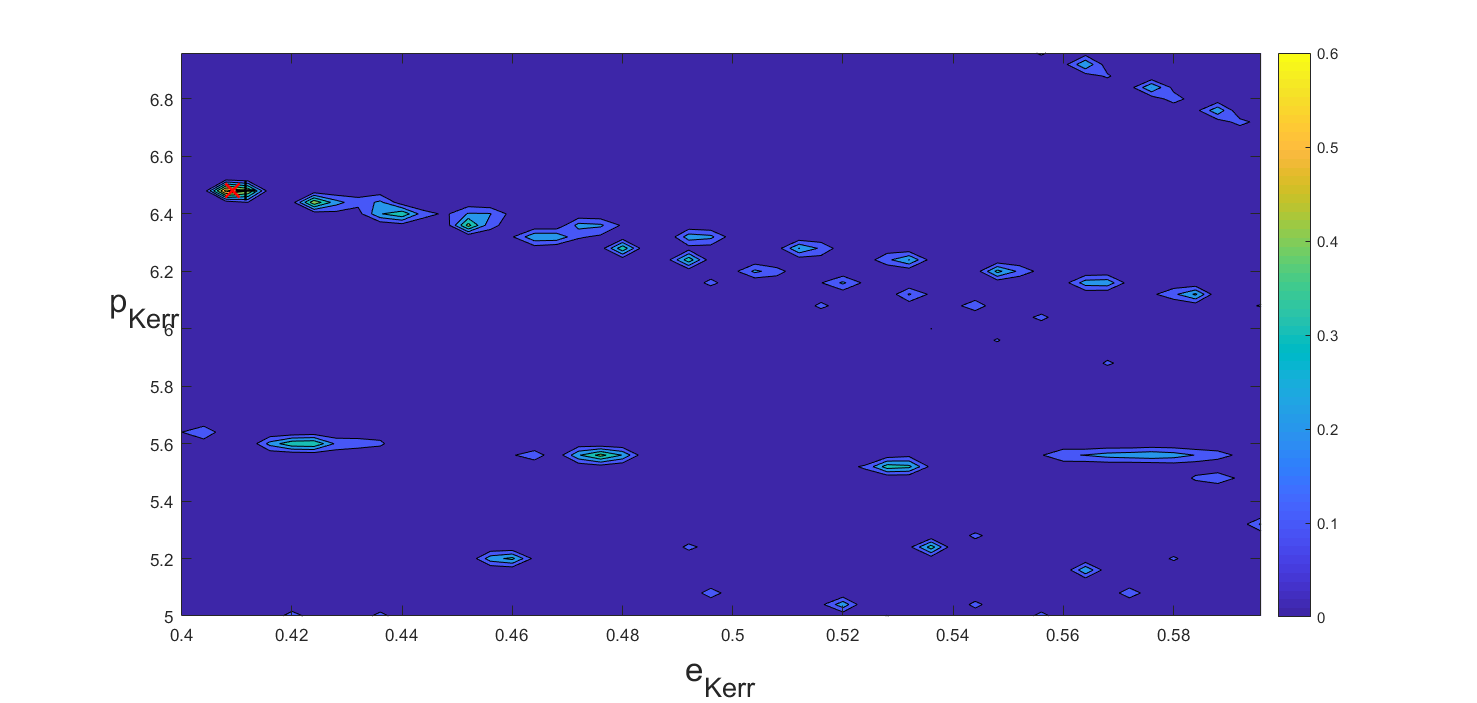
\includegraphics[width=8cm]{OLdist.png}
	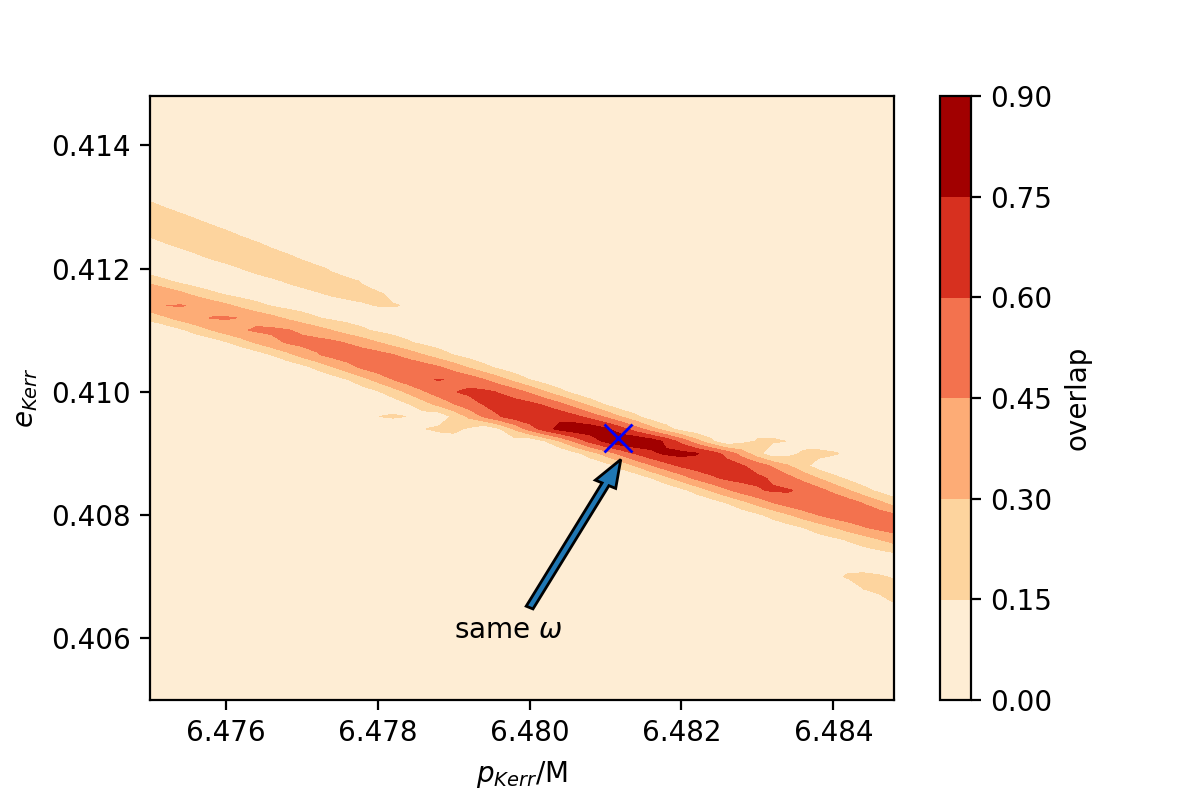
\includegraphics[width=8cm]{OLdist2.png}
	
	\caption{Distribution of overlap between waveform of ($\delta_1,\, a,\, M,\, e,\, p$) = (0.2, 0.5, $2 \times 10^5 $, 0.5, 6) and waveforms of ($\delta_1,\, a,\, M,\, e,\, p$) =(0, 0.5, $2 \times 10^5 $, $e_{Kerr}$, $p_{Kerr}$) on ($e_{Kerr}$, $p_{Kerr}$) plane. Red cross mark: same $\omega^{(t)}$ at ($e_{Kerr}$, $p_{Kerr}$) = (0.409248, 6.481170), overlap is 0.8912. The grid size is 50*50.}
	\label{overlapdist}
\end{figure}

According to Ref. \cite{sameOmg}, orbits with same orbital frequency $\omega_r$ and $\omega_\phi$ can generate gravitational waveforms potentially confused with non-Kerr signals. Therefore the overlap between a non-Kerr waveform and several Kerr waveforms should have a local maximum around the parameter leading to same orbital frequency. Here we check this result by looking at overlaps between waveform of ($\delta_1,\, a,\, M,\, e,\, p$) = (0.2, 0.5, $2 \times 10^5 $ , 0.5, 6) and of ($\delta_1,\, a,\, M,\, e,\, p$) = (0, 0.5, $2 \times 10^5 $ , $e_{Kerr}$, $p_{Kerr}$) with varying $e_{Kerr}$ and $p_{Kerr}$. First we look at overlap distribution on a relatively large range of (e, p). Then we search near ($e_{Kerr}$, $p_{Kerr}$) with same orbital frequency, as shown in Fig. \ref{overlapdist}. 

	\begin{figure}[!htb]
	\centering
	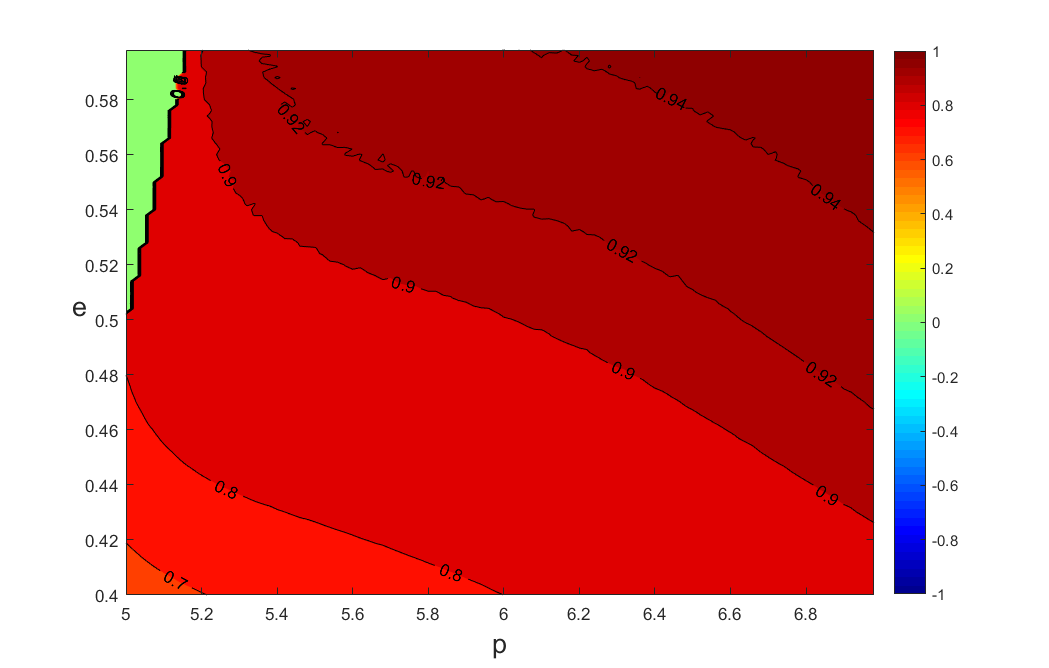
\includegraphics[width=16cm]{ep_best_dist.png}
	
	\caption{distribution of overlap between waveform of ($\delta_1,\, a,\, M,\, e,\, p$) = (0.2, 0.5, $2 \times 10^5 $ , $e$, $p$) and Kerr waveform with identical $\omega^{(t)}$ by varying $e_{Kerr},\, p_{Kerr}$. The grid size is 50*50. The green region is unstable orbits.}
	\label{epdist}
\end{figure}	

	\begin{figure}[!htb]
	\centering
	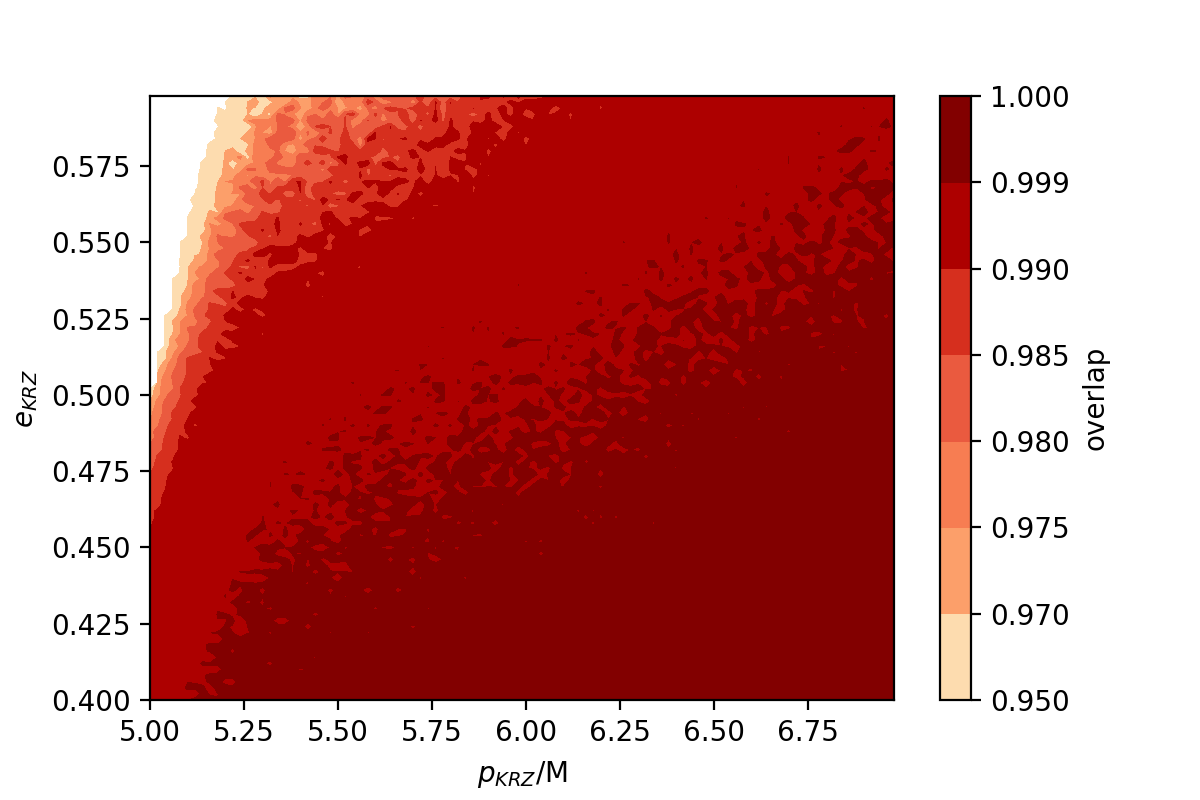
\includegraphics[width=16cm]{FF_am.png}
	
	\caption{distribution of overlap between waveform of ($\delta_1,\, a,\, M,\, e,\, p$) = (0.2, 0.5, $2 \times 10^5 $ , $e$, $p$) and Kerr waveform with identical $\omega^{(t)}$ by varying $M_{Kerr},\, a_{Kerr}$. The grid size is 50*50. The blank region is unstable orbits.}
	\label{amdist}
\end{figure}	

Since metric deformation is more evident near BH horizon, we look at waveforms generated by trajectories close to innermost bound orbit. We compare waveforms of ($\delta_1,\, a,\, M,\, e,\, p$) = (0.2, 0.5, $2 \times 10^5 $ , $e$, $p$) and Kerr orbits varying $(e,p)$ or $(M,a)$ in a 50*50 grid of $(e,p)$. Contour plots of waveform overlap when varying $(e,p)$ and $(M,a)$ are shown in Fig. \ref{epdist} and \ref{amdist}. The confusion problem exists when varying $(M,a)$ for most region we considered. 

#degenerate

#上下限

\subsection{Inclined orbit}
\label{p_3d}



Note that the difference between equating $\omega^{(t)}$, orbital frequency with respect to coordinate time, and $\omega^{(\tau)}$, orbital frequency with respect to proper time, can be significant. From Fig. \ref{overlapdist} it is explicit that the same orbital frequency with respect to t can result in almost the largest overlap while the same orbital frequency with respect to $\tau$ cannot. In Kerr spacetime, the expression for $\omega^{(t)}$ and $\omega^{(\tau)}$ are given in \cite{tOmg} and \cite{tauOmg}.


This result is explicit by looking at the waveforms over a relatively long time (here about $50000M$), as shown in Fig. \ref{kkwave}. 


	
	\begin{figure}[!htb]
		\centering
		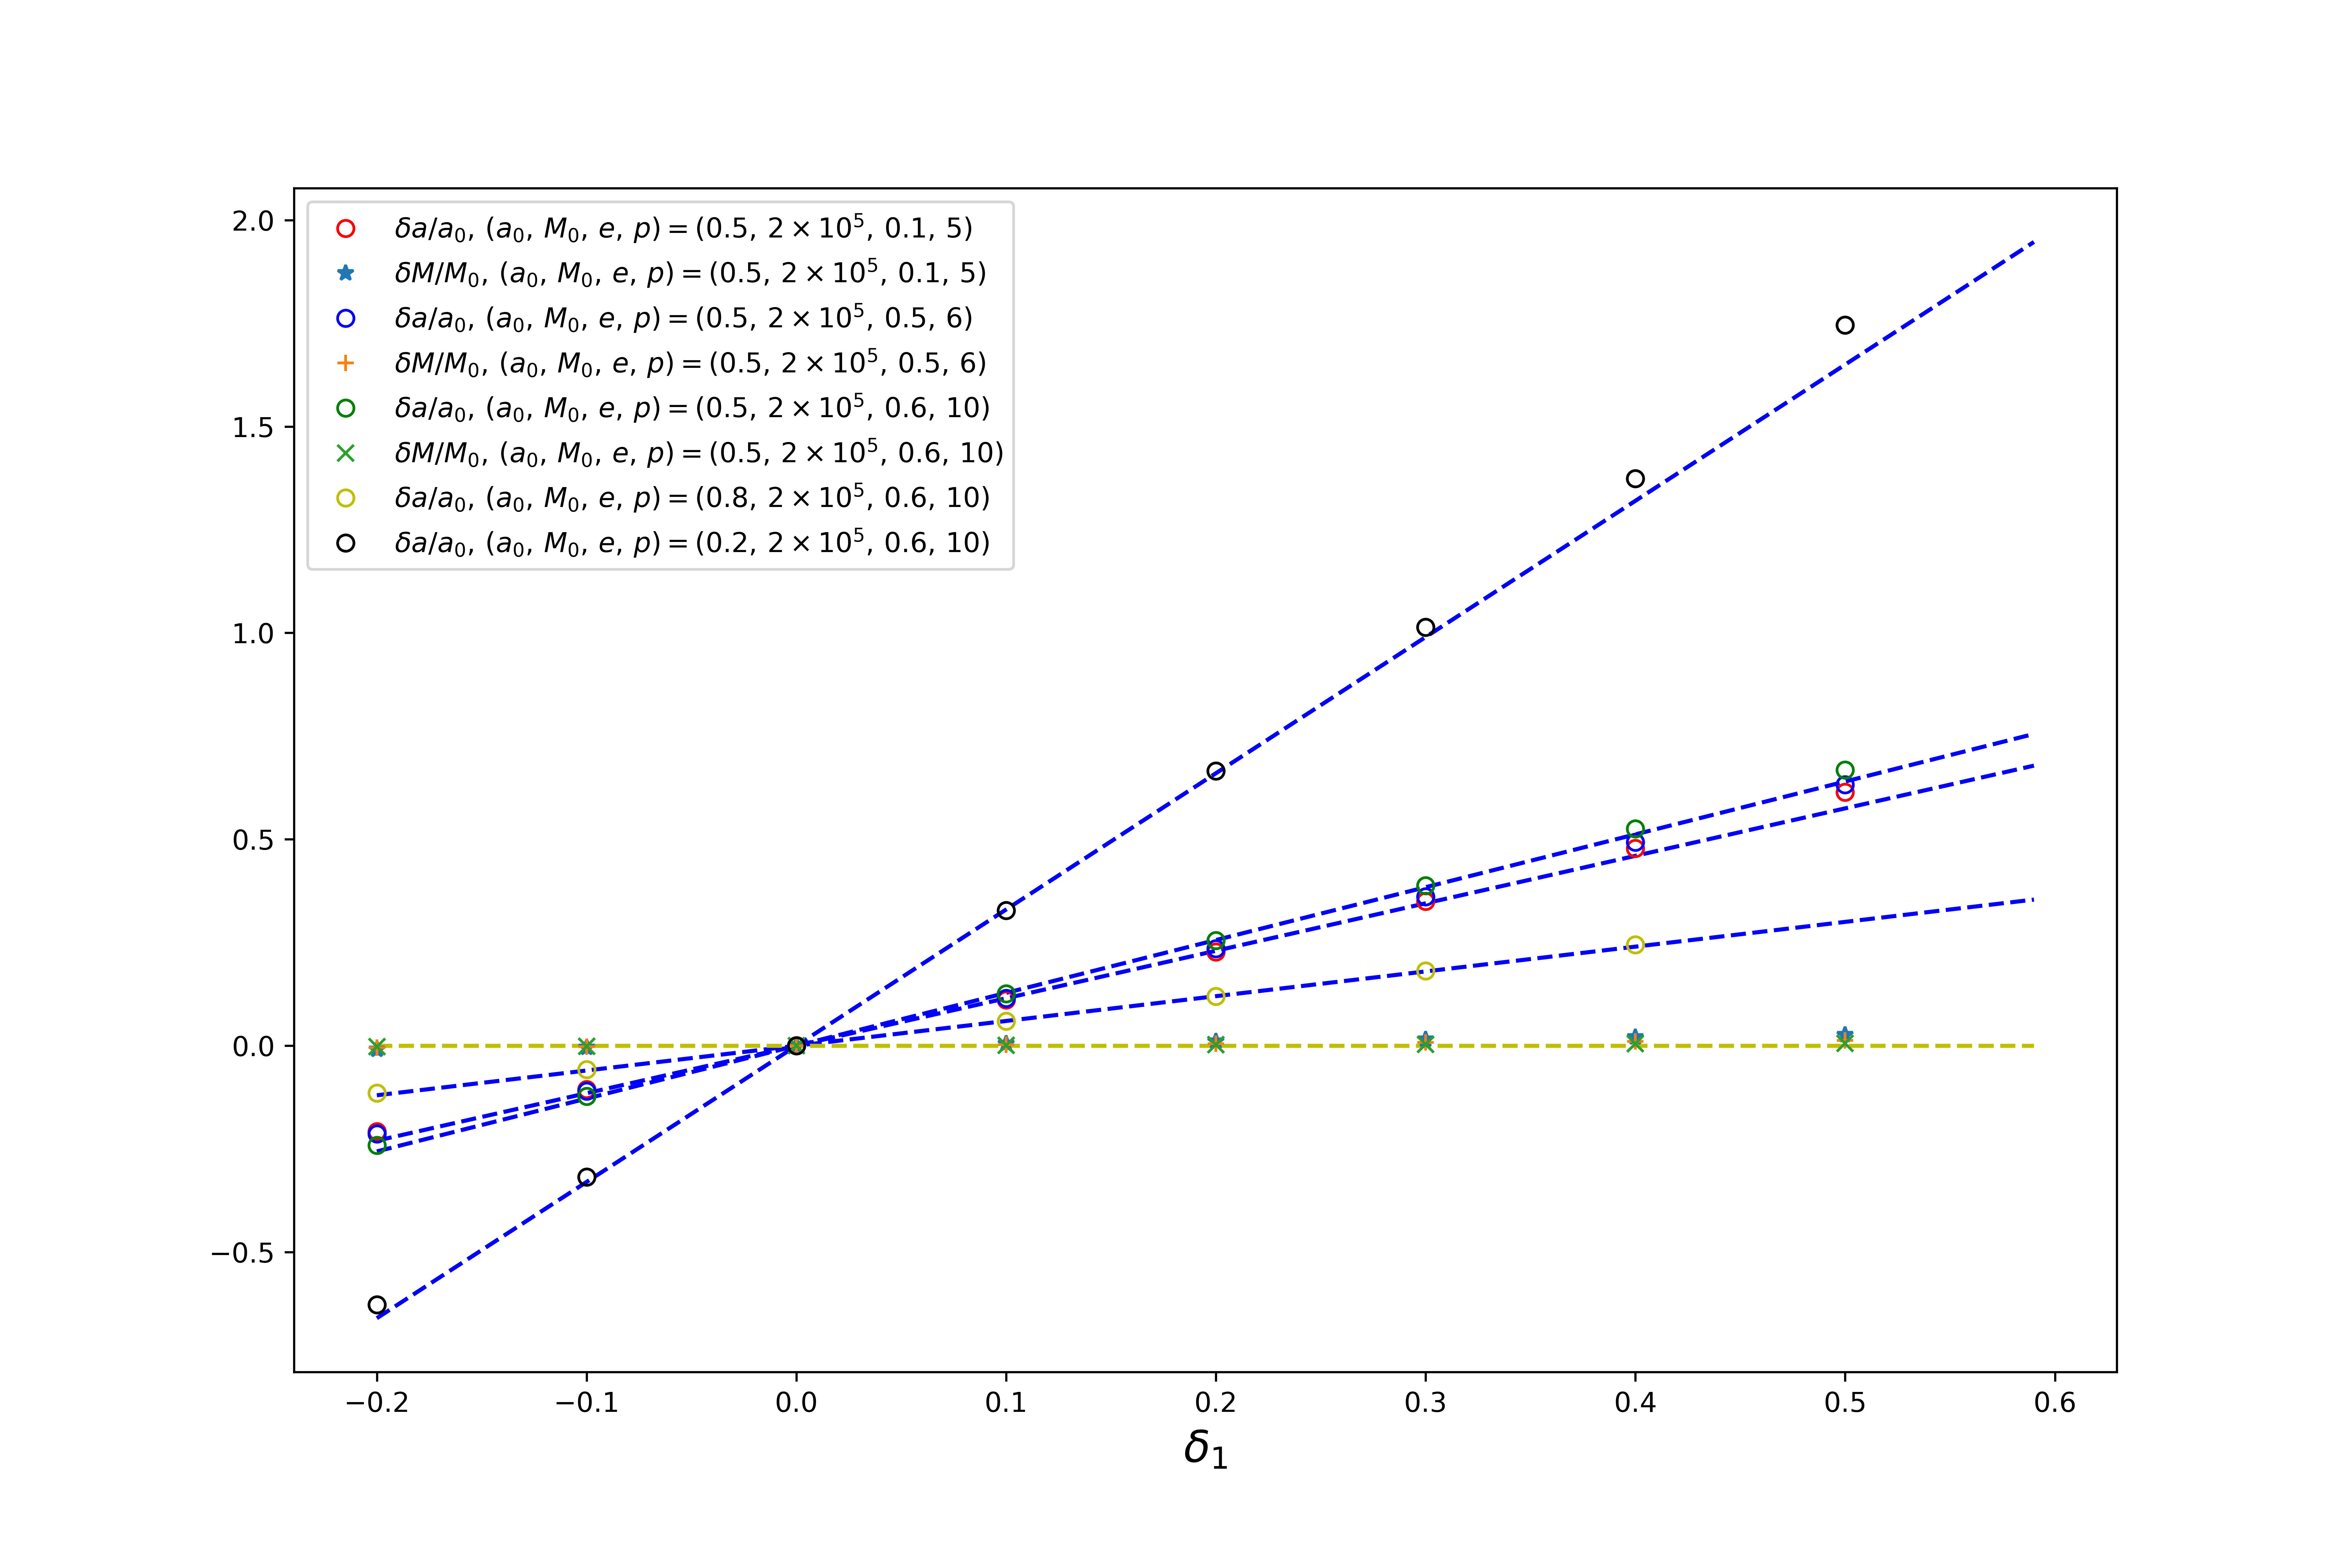
\includegraphics[width=16cm]{d1_spin_linear.png}
		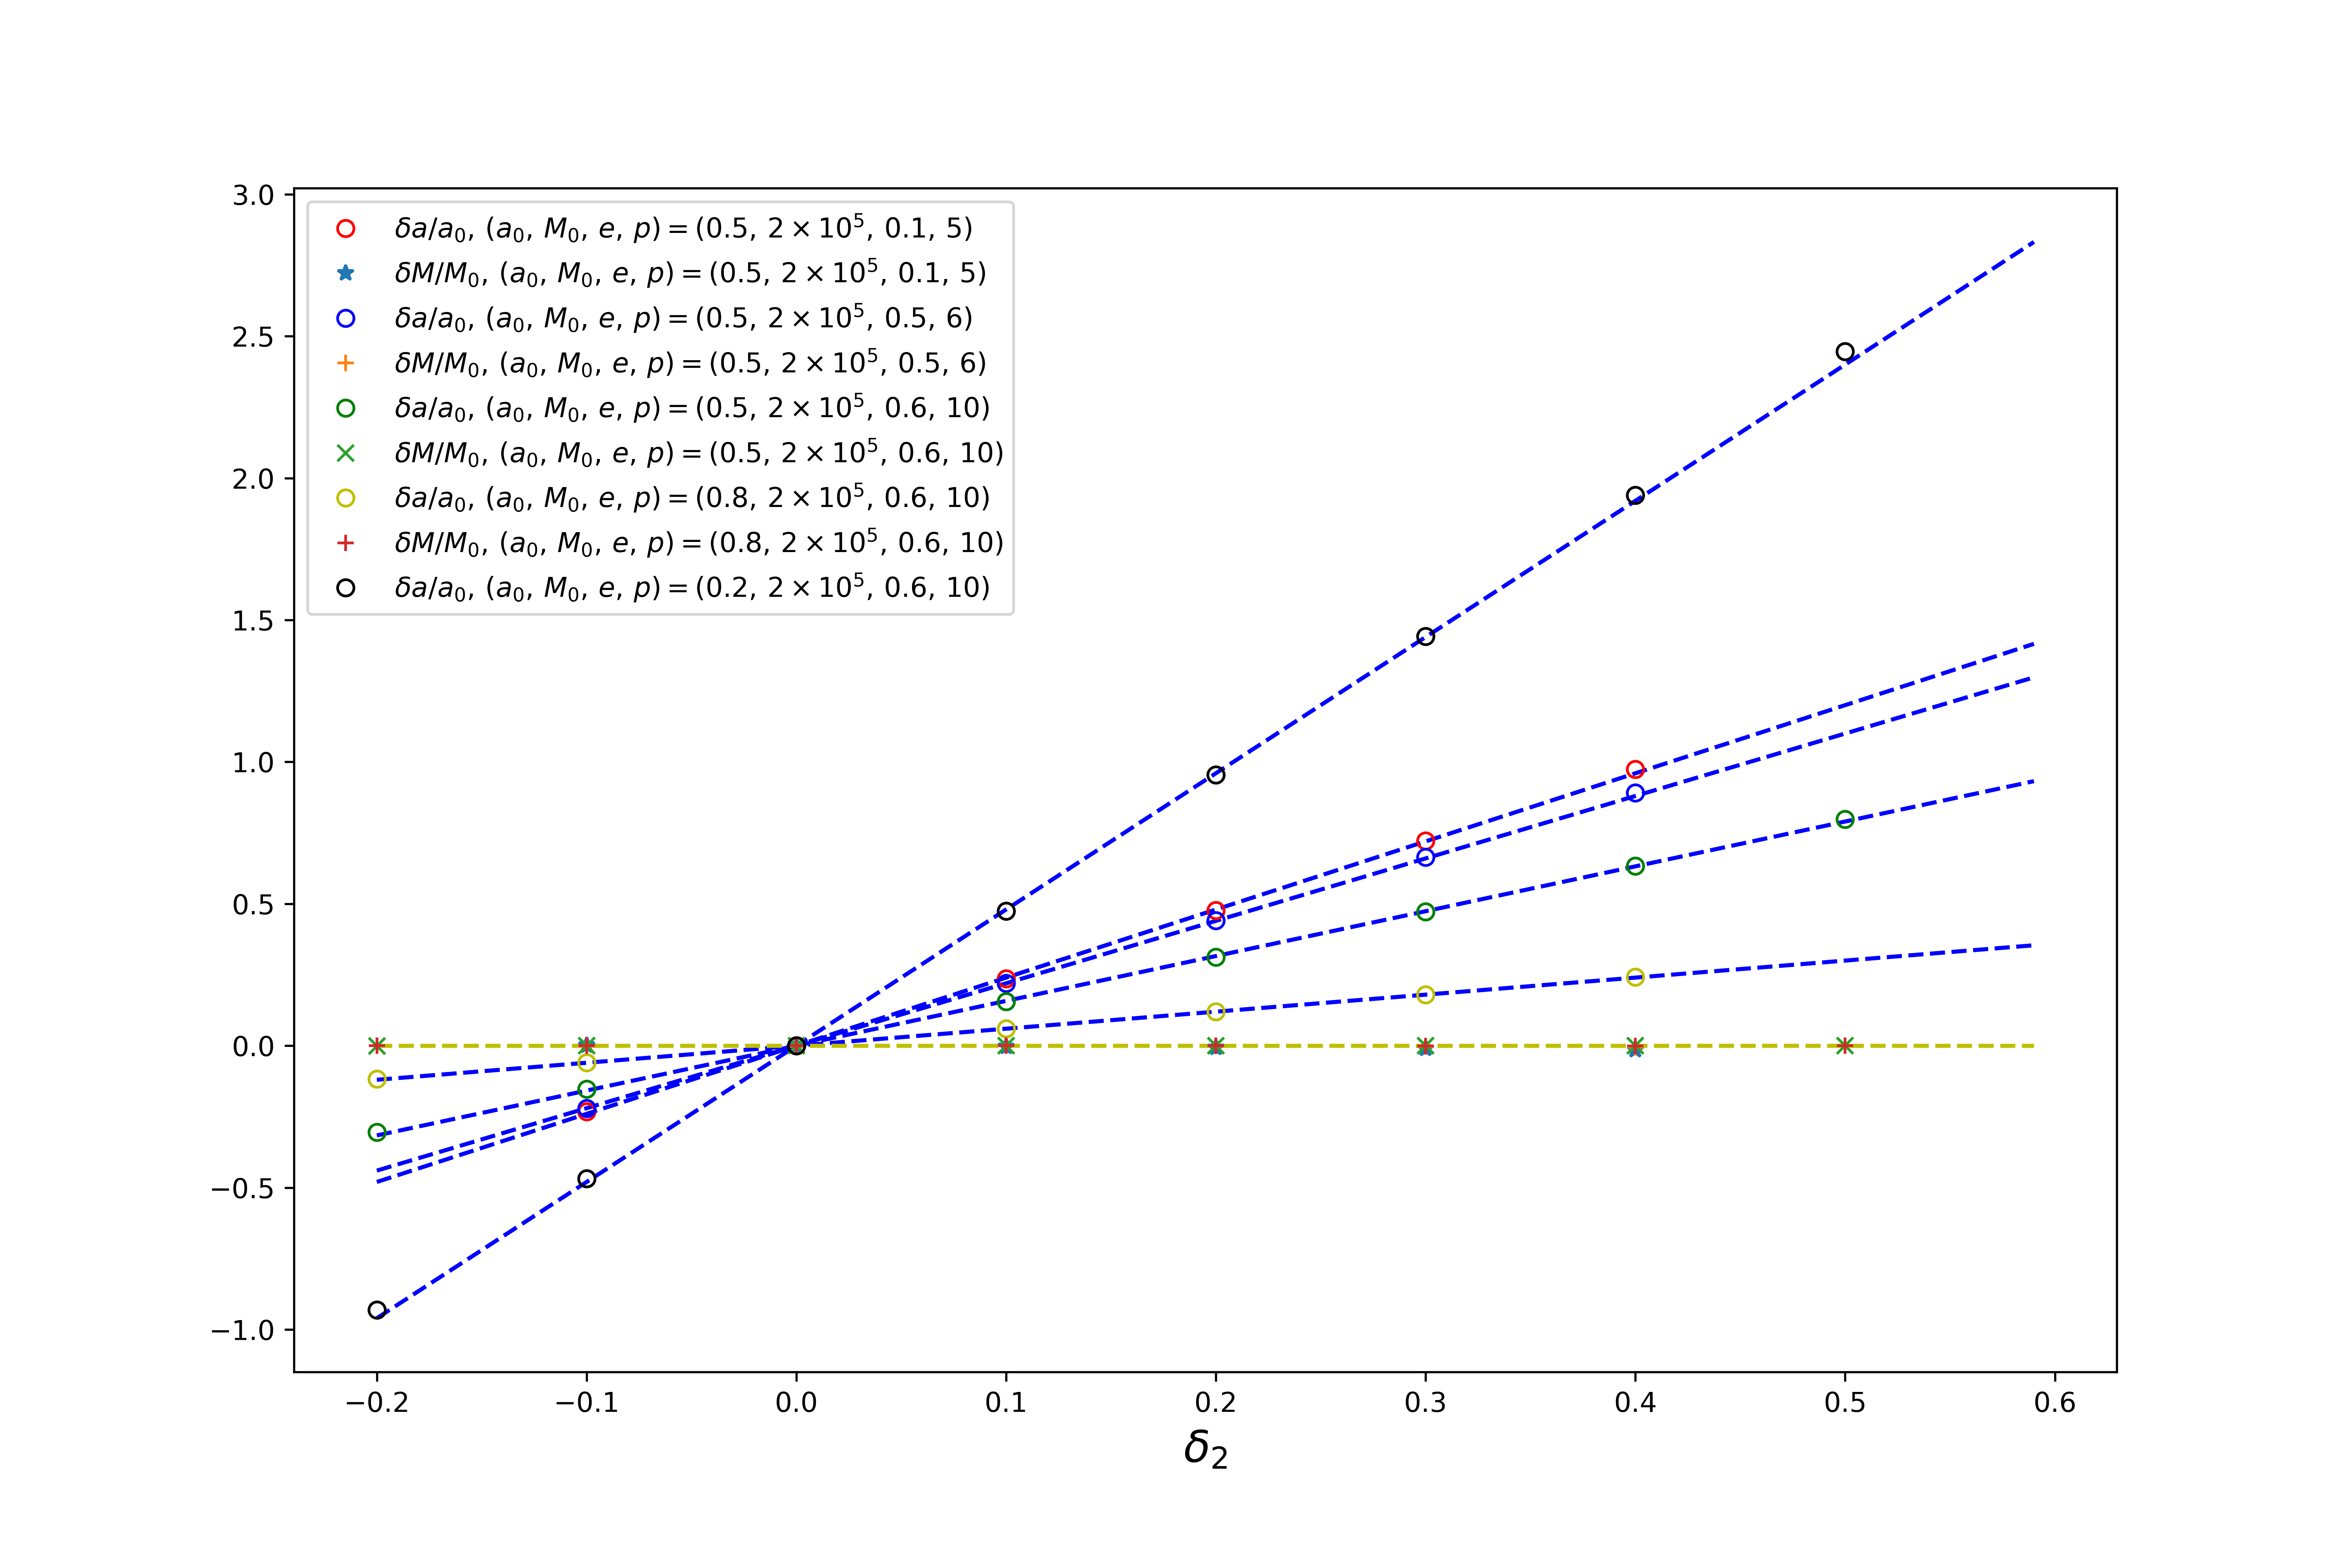
\includegraphics[width=7cm]{d2_spin_linear.png}
		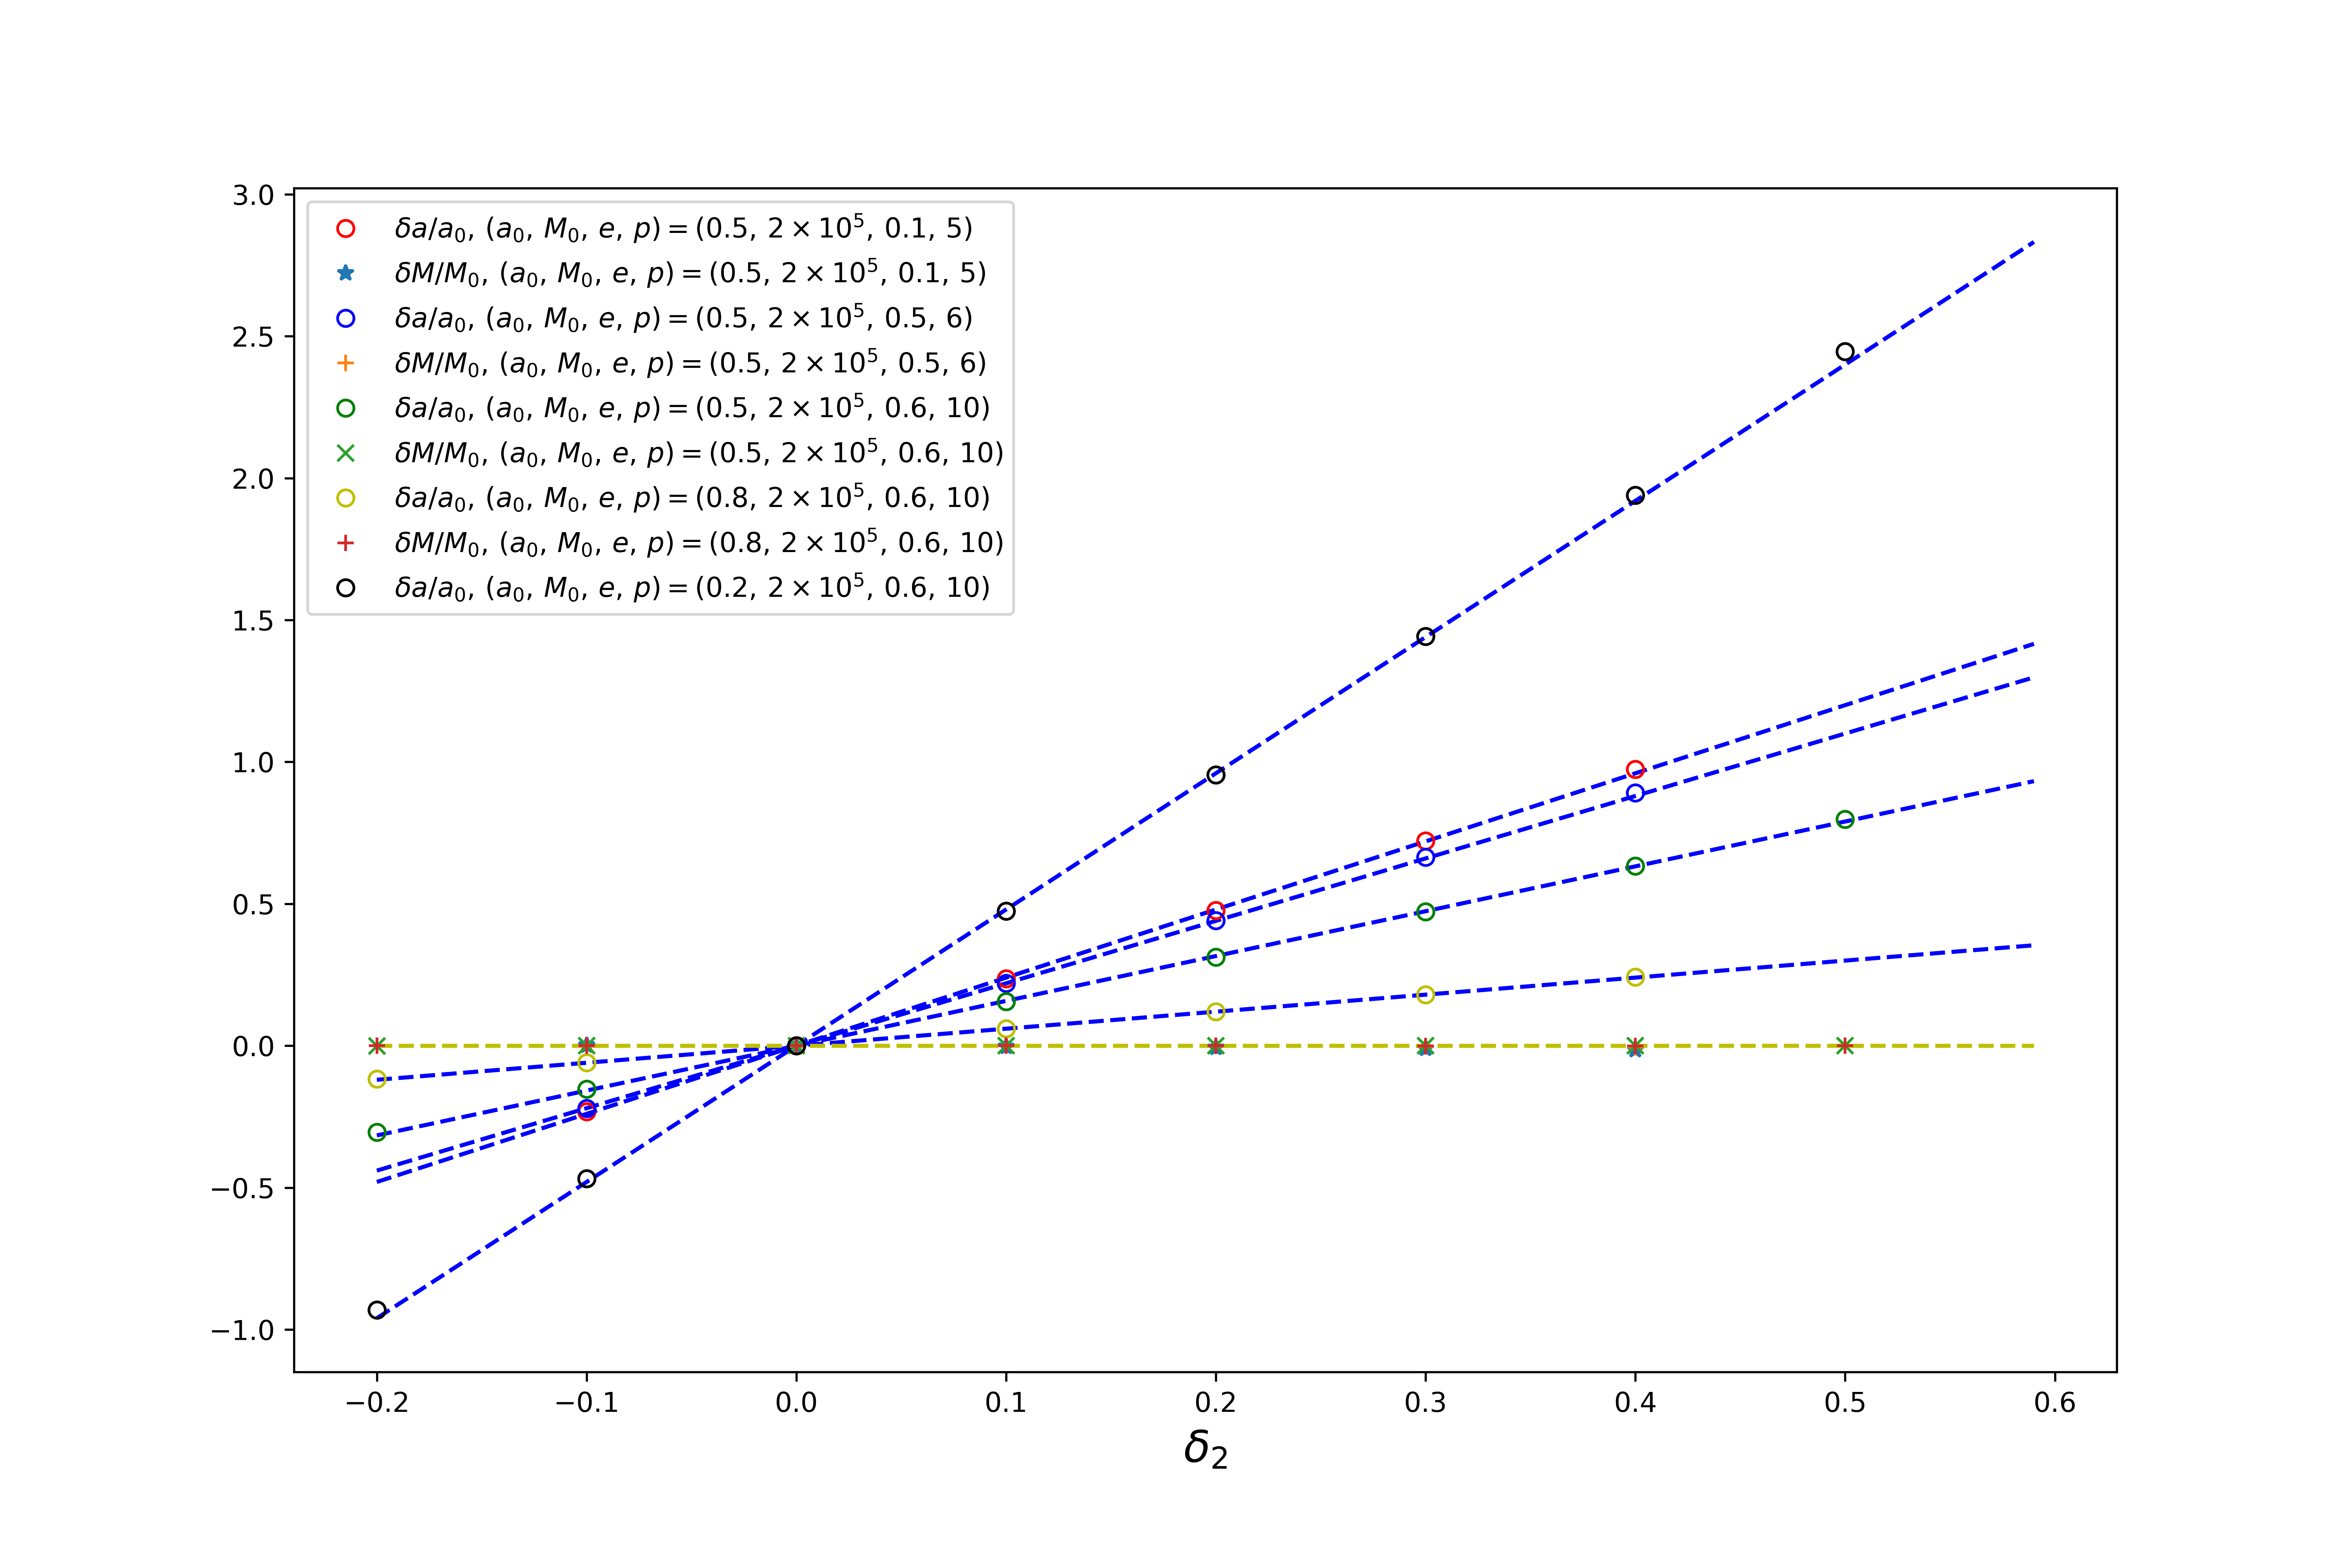
\includegraphics[width=7cm]{d2_spin_linear.png}
		\caption{relation between relative varied spin/Mass and , for upper panel: $\delta_1$, for lower panel: $\delta_2$, when varying spin and mass to get identical $\omega^{(t)}$. The relative varied mass $\delta M/ M_0$ is almost zero compared to relative varied spin $\delta a/ a_0$. Moreover, $\delta a/ a_0$ show linear behavior with respect to deformation parameters.}
		\label{da_linear}
	\end{figure}

\begin{figure}[!htb]
	\centering
	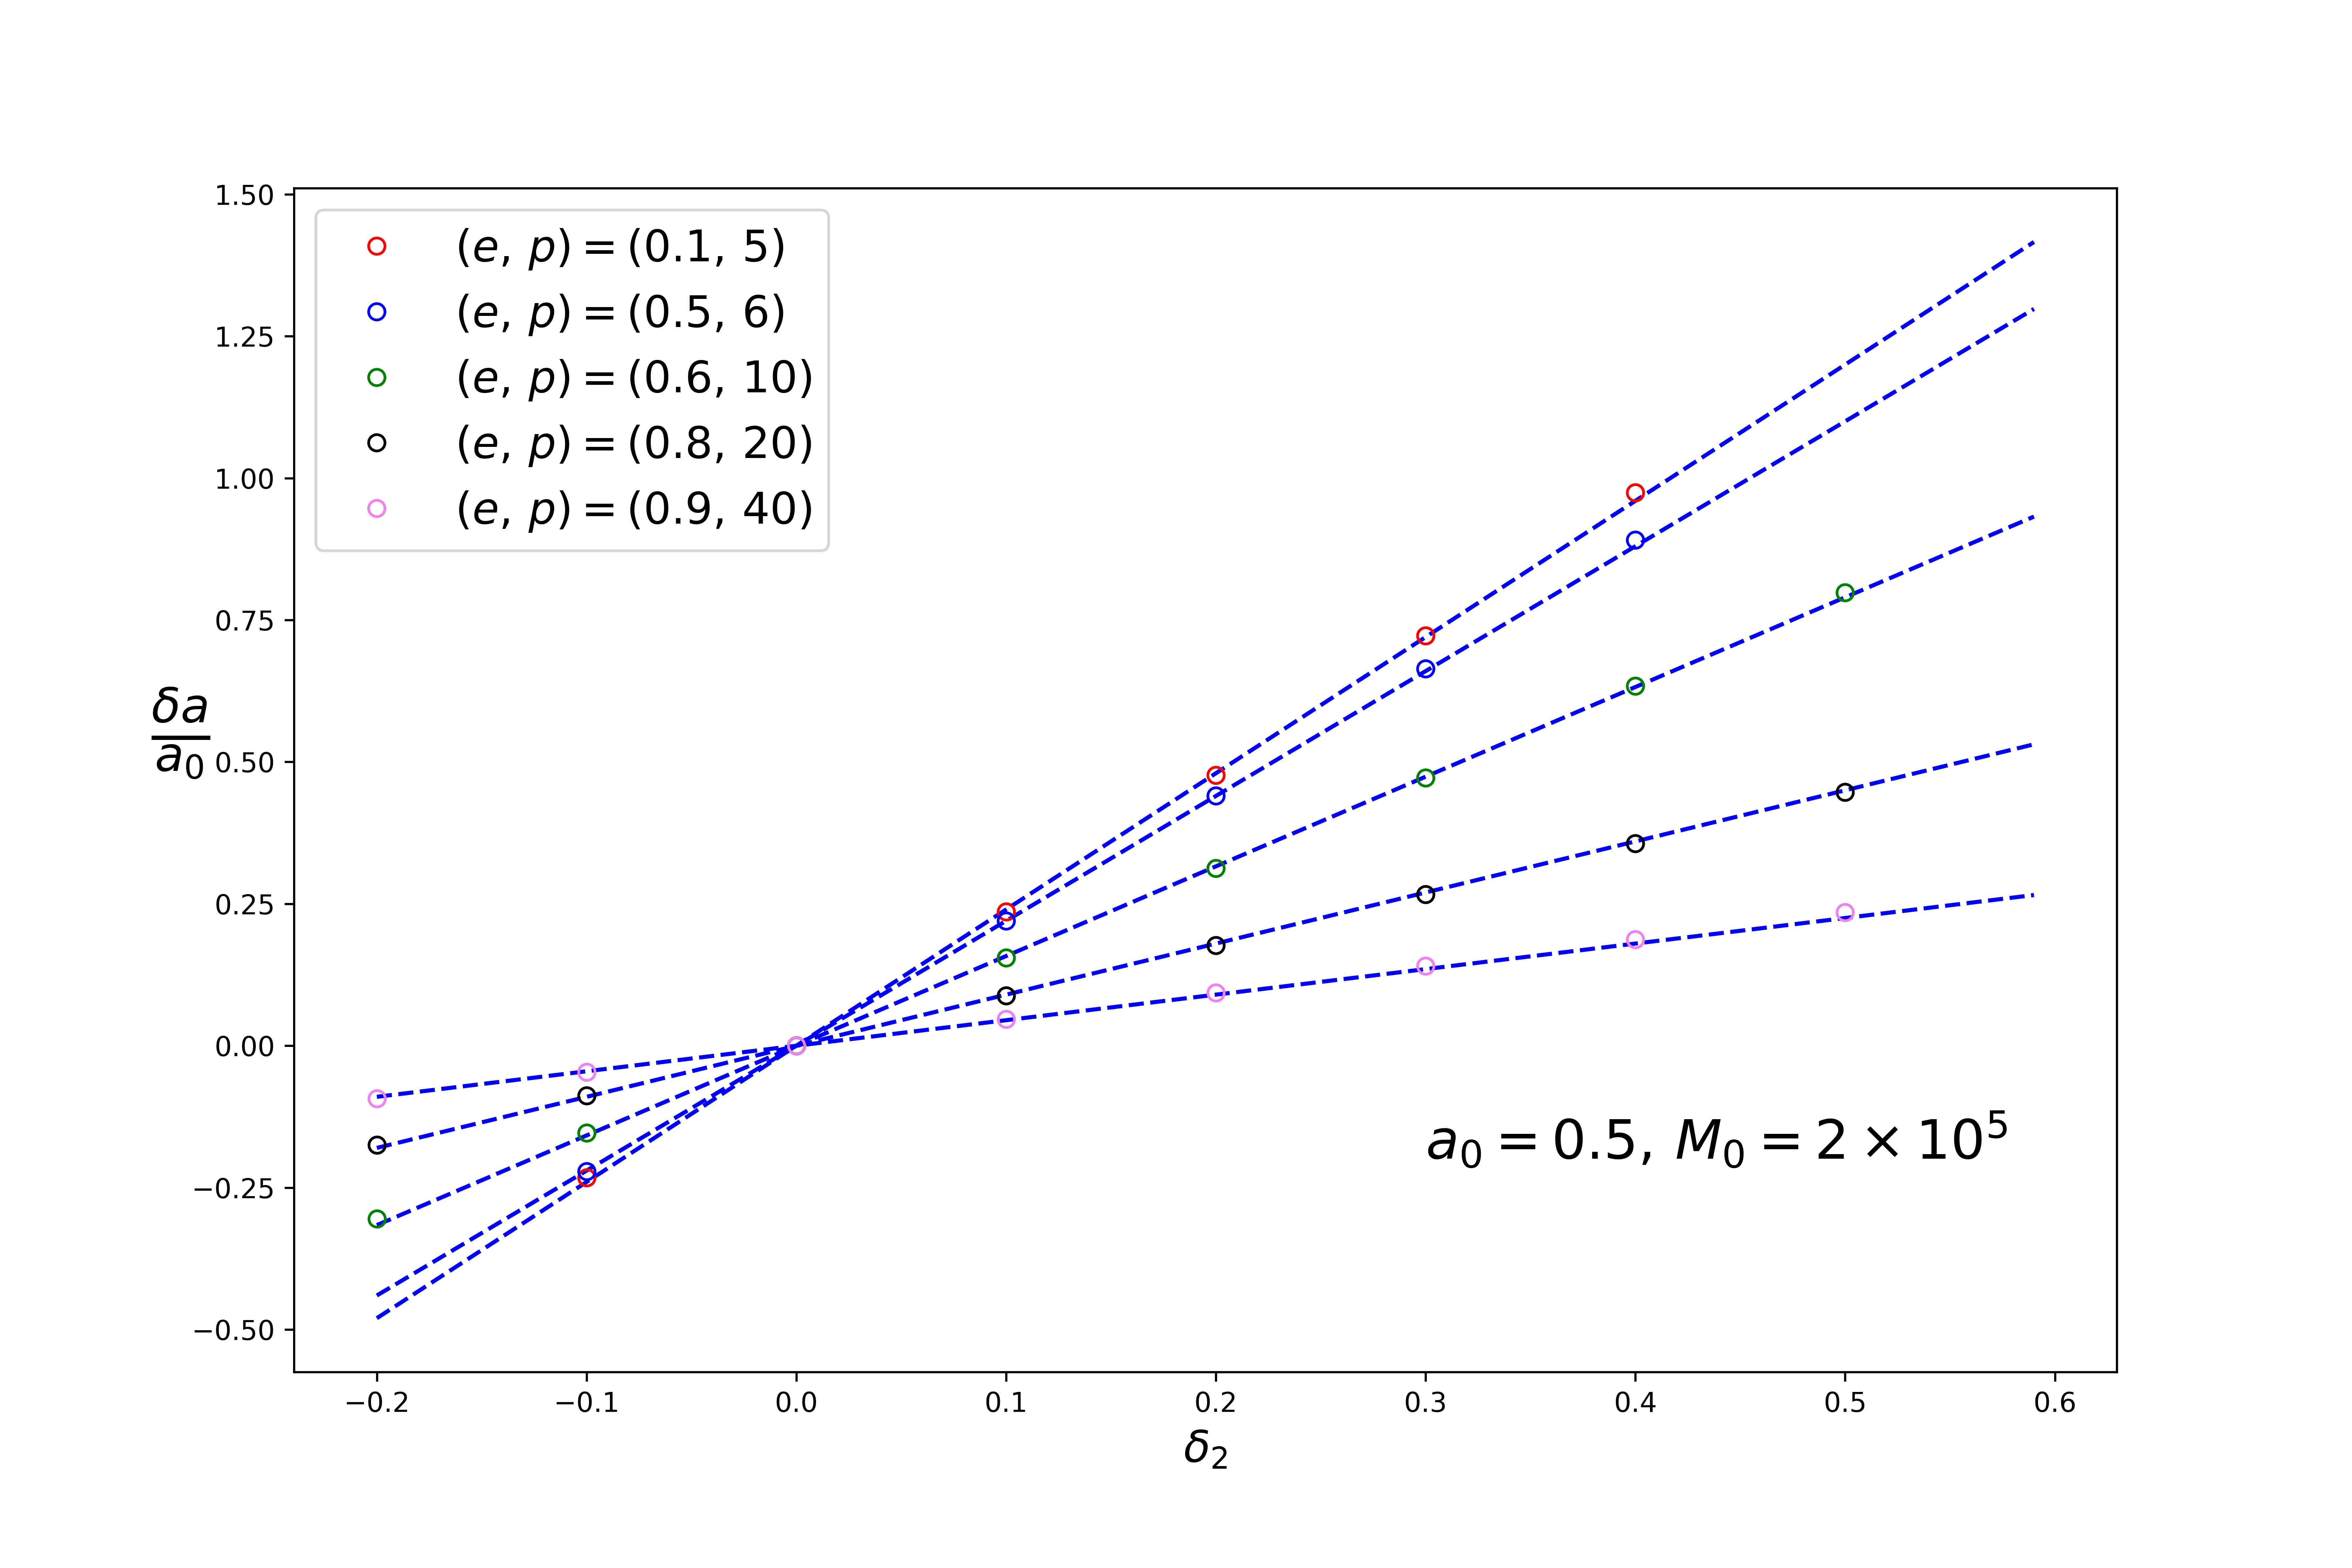
\includegraphics[width=16cm]{d2_deltaspin_ep.png}

	\caption{influence of (e, p) on the slope of the aforementioned linear relation between $\delta a/a_0$ and deformation parameter. }
	\label{ep_slope}
\end{figure}

\begin{figure}[!htb]
	\centering
	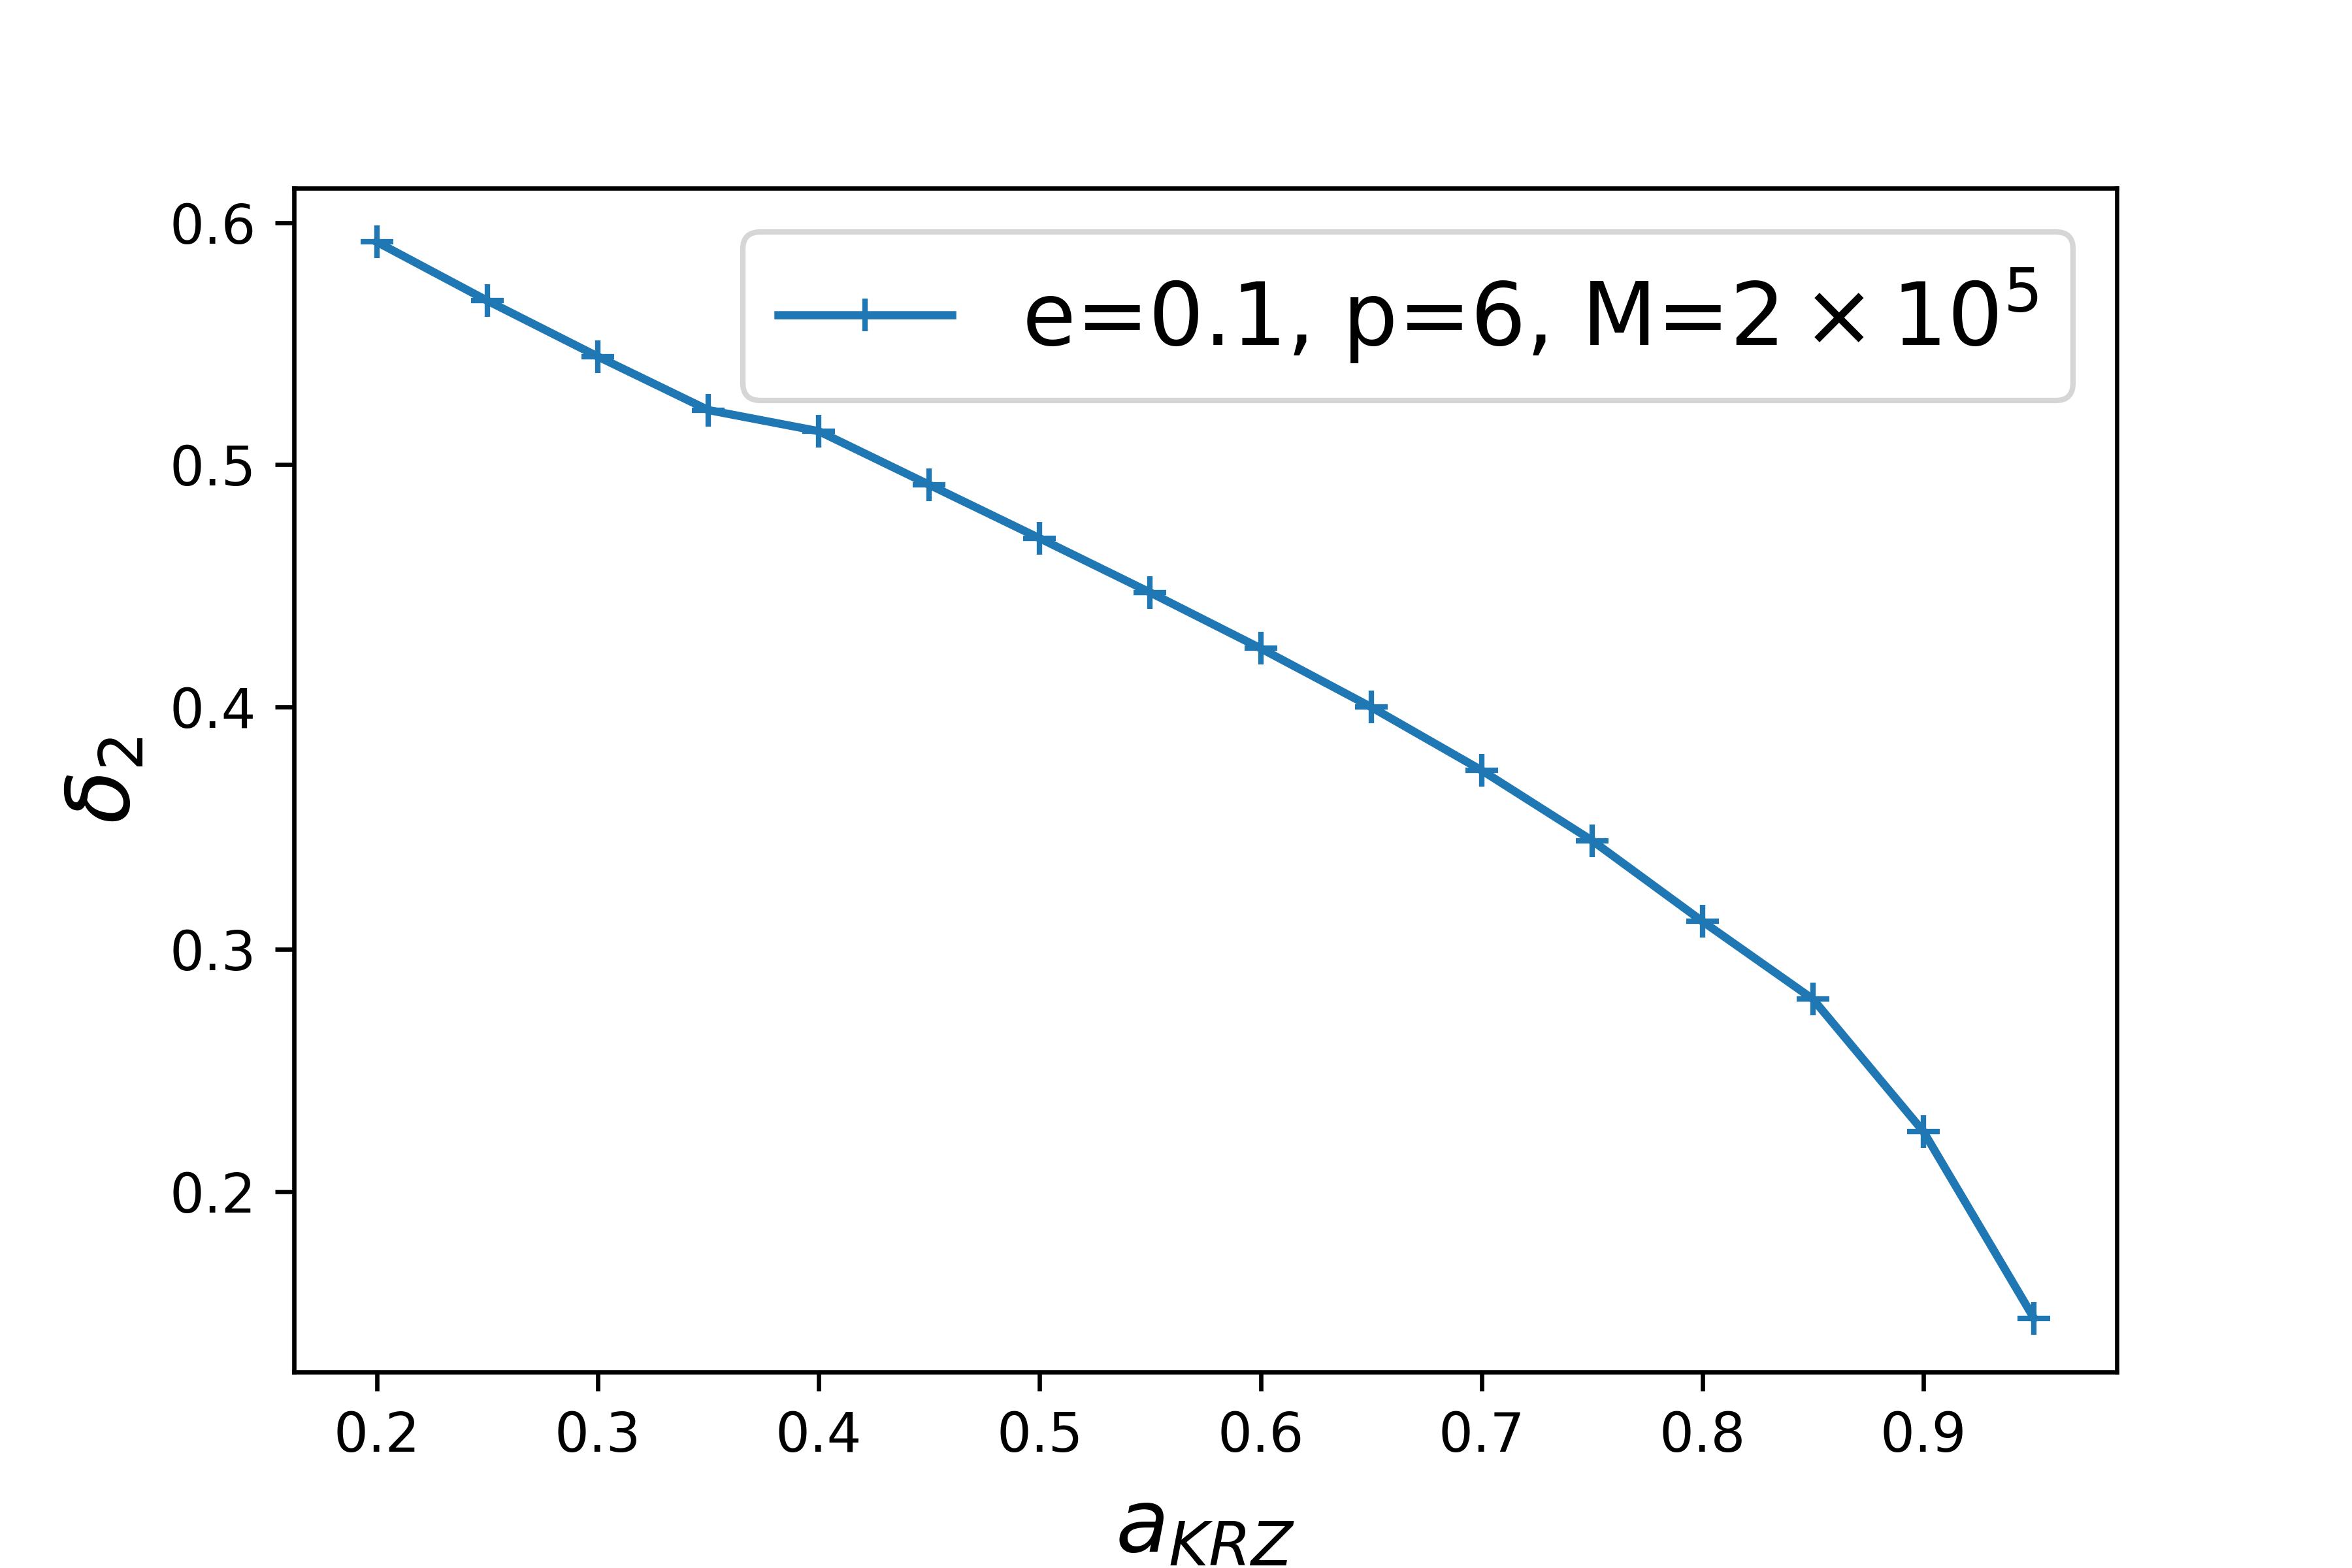
\includegraphics[width=16cm]{limit_d2_e01_p6.png}
	
	\caption{upper limit of deformation $\delta_2$ for each spin, waveform of which parameter can be recovered by varying spin and mass under Kerr metric. The waveform have (e, p)=(0.1, 6)}
	\label{d2limit}
\end{figure}
Therefore we regard waveforms in Kerr spacetime with same orbital frequencies with respect to proper time as best matches to waveforms in non-Kerr space time under KRZ parametrization.

Fig. shows the overlap distribution...

As Fig. suggest, the confusion problem still exists in KRZ parametrization. In terms of gravitational waves, the deformation parameters are kind of degenerated with spin in Kerr spacetime. This resulted can also be found by looking at covariance matrix as discussed in next section
\section{Constraints on deformation parameter by future LISA task}

\bibliography{citation}
\bibliographystyle{plain}
\end{document}